\documentclass[a4paper,14pt]{extarticle}
\usepackage[utf8]{inputenc}
\usepackage[russian]{babel}
\usepackage{graphicx}
\usepackage[top=0.8in, bottom=0.8in, left=0.8in, right=0.8in]{geometry}
\usepackage{pgfplots}
\usepackage{amsmath}
\usepackage{setspace}
\usepackage{titlesec}
\usepackage{float}
\usepackage{chngcntr}
\usepackage{pgfplots}
\usepackage{amsfonts}
\usepackage{pgfplotstable}
\usepackage{multirow}
\usepackage{karnaugh-map}
\usepackage{tikz,xcolor}
\usepackage{listings}
\usepackage{txfonts}

\titleformat{\section}[hang]
  {\bfseries}
  {}
  {0em}
  {\hspace{-0.4pt}\large \thesection\hspace{0.6em}}
  
\titleformat{\subsection}[hang]
  {\bfseries}
  {}
  {0em}
  {\hspace{-0.4pt}\large \thesubsection\hspace{0.6em}}

\newcommand{\nx}{\overline{x}}
\newcommand{\p}{0.31}
\newcommand{\scale}{1.4}

\counterwithin{figure}{section}
\counterwithin{equation}{section}
\counterwithin{table}{section}

\lstdefinestyle{CStyle}{
    basicstyle=\footnotesize,
    breakatwhitespace=false,         
    breaklines=true,                 
    captionpos=b,
    %caption = {[Текст] программа},
    caption = {},              
    keepspaces=true,                 
    numbers=left,                    
    numbersep=5pt,                  
    showspaces=false,                
    showstringspaces=false,
    showtabs=false,                  
    tabsize=2,
    language=C
}

\begin{document}
\begin{titlepage}
\centering
\small Балтийский государственный технический университет «Военмех» им. Д.Ф.Устинова \\
\vspace{3cm}
\normalsize Кафедра И5\\
«Информационные системы и программная инженерия»\\
\vspace{3cm}
\textbf{Практическое задание №2}\\
по дисциплине Основы программирования на тему\\ 
\textbf{«Ветвления и циклы»}\\
\begin{center}
{\large\bf Вариант 14}
\end{center}
\vfill

\begin{flushleft}
\textbf{Выполнил:}
\hfill {Мальцев А.С.} \\
\hfill {Группа И595} \\
\vspace{1cm}
\textbf{Преподаватель:}
\hfill {Лазарева Т.И.} \\
\end{flushleft}
\vspace{3cm}

{\centering Санкт-Петербург \\ 
\vspace{0.15cm}
2019}
\end{titlepage}

\section{Цель работы}
Познакомиться с функциями из математической библиотеки, освоить операции отношения и логические операции, научиться грамотно программировать базовые алгоритмические структуры «ветвление» и «цикл».
\setcounter{page}{2}

\section{Ход работы}
\subsection{Задание 1}
Вычислить значение функции\\
\begin{equation*}
f(m,n) = 
 \begin{cases}
   \displaystyle\frac 5 m - \frac n 5 \text{, если $ n > -5, m \neq 0$}\\
   3m + n^2 \text{, если $ n \leq -5$}\\
   2mn \text{ в остальных случаях}
 \end{cases}
\end{equation*}
используя тернарный оператор.\\
\textit{Исходные данные:} так как значения m и n могут быть любыми, объявим соответствующие переменные типа double.\\
\textit{Результирующие данные:} значение функции f также типа double.\\
\begin{center}
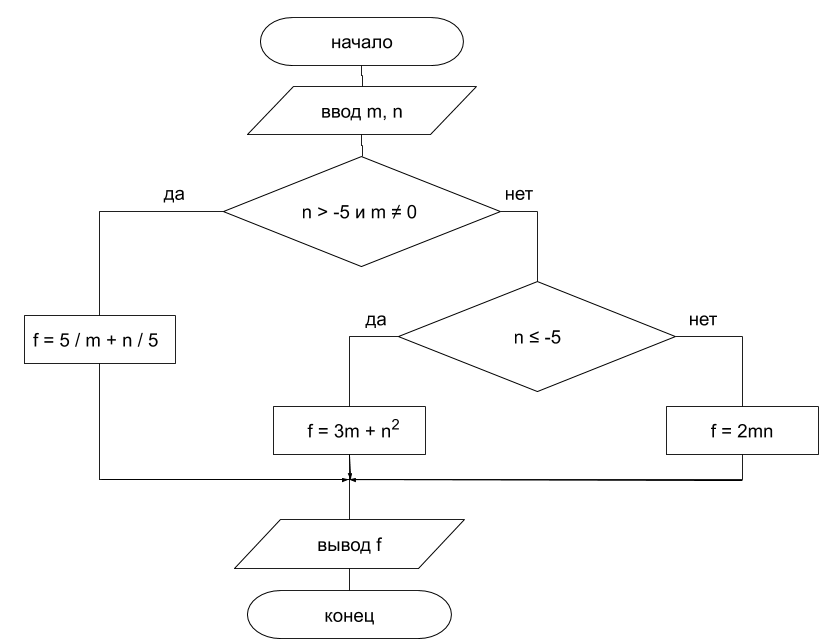
\includegraphics[scale=0.6]{lab2-1.png}
Схема программы
\end{center}
\lstinputlisting[language=c, frame=single, caption=Программа первого задания, style=CStyle]{../firstTask.c}
\begin{center}
Текст программы
\end{center}
\begin{center}
\begin{tabular}{|l|l|}
\hline
\multicolumn{1}{|c|}{Исходные данные}& \multicolumn{1}{|c|}{Вывод программы}\\
\hline
m = 2, n = 4 & f = 1.700000\\
m = 3, n = -8 & f = 73.000000\\
m = 0, n = 0 & f = 0.000000\\
\hline
\end{tabular}\\
\vspace{0.3cm}
Результаты тестирования
\end{center}

\subsection{Задание 2}
Вычислить значение функции
$S = \displaystyle\frac{ \sin \alphaup^3 + 2\cos^2\betaup }{\sqrt{2,5\alphaup + 3\betaup  + \sqrt{2}}\ln \betaup }$\\
\textit{Исходные данные:} типы $\alphaup$ и $\betaup$ не указаны в задании, поэтому будут double.\\
\textit{Результирующие данные:} значение S также типа double.\\
\textit{Предварительные вычисления:} подкоренное и подлогарифмическое выражения должны быть больше нуля.\\
\vspace{0.5cm}
\begin{center}
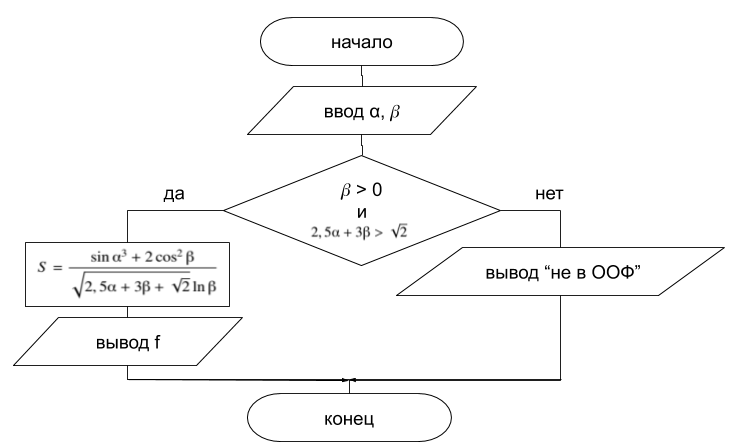
\includegraphics[scale=0.6]{lab2-2.png}
Схема программы
\end{center}
\lstinputlisting[language=c, frame=single, caption=Программа второго задания, style=CStyle]{../secondTask.c}
\begin{center}
Текст программы
\end{center}
\begin{center}
\begin{tabular}{|l|l|}
\hline
\multicolumn{1}{|c|}{Исходные данные}& \multicolumn{1}{|c|}{Вывод программы}\\
\hline
a = 2, b = 2 & s = 0.546926\\
a = -3, b = 10 & s = 0.040116\\
a = 5, b = -2 & Недопустимое значение\\
a = 10, b = 6 & Недопустимое значение\\
\hline
\end{tabular}\\
\vspace{0.3cm}
Результаты тестирования
\end{center}

\subsection{Задание 3}
В финале шашечной партии остались белая дамка и две черные пешки, позиции которых известны. Ход белых. Сможет ли дамка «срубить» хотя бы одну пешку?\\
\textit{Исходные данные:} типы x1, x2, x3, y1, y2, y3 не указаны в задании, поэтому будут int, т.к. они содержат координаты шашек на доске.\\
\textit{Результирующие данные:} Отдельной переменной не требуется.\\
\begin{center}
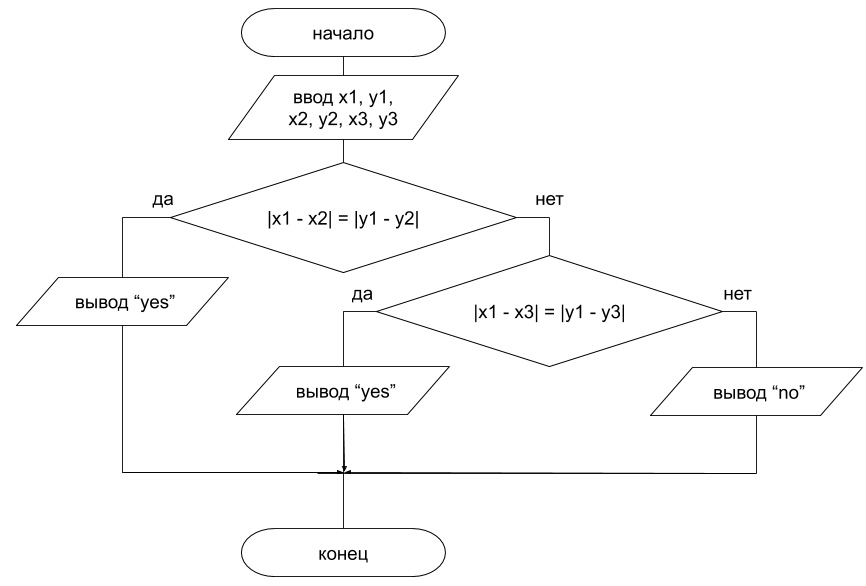
\includegraphics[scale=0.6]{lab2-3.png}\\
Схема программы
\end{center}
\lstinputlisting[language=c, frame=single, caption=Программа третьего задания, label=lab2_2, style=CStyle]{../thirdTask.c}
\begin{center}
Текст программы
\end{center}
\begin{center}
\begin{tabular}{|l|l|}
\hline
\multicolumn{1}{|c|}{Исходные данные}& \multicolumn{1}{|c|}{Вывод программы}\\
\hline
x1 = 1, y1 = 1, x2 = 6, y2 = 4, x3 = 2, y3 = 8 & no\\
x1 = 4, y1 = 4, x2 = 7, y2 = 7, x3 = 1, y3 = 5 & yes\\
x1 = 1, y1 = 5, x2 = 2, y2 = 3, x3 = 3, y3 = 8 & no\\
x1 = 2, y1 = 6, x2 = 4, y2 = 8, x3 = 6, y3 = 7 & yes\\
\hline
\end{tabular}\\
\vspace{0.3cm}
Результаты тестирования
\end{center}

\subsection{Задание 4}
Составить программу для определения, в каких двузначных числах удвоенная сумма цифр равна их произведению.\\
\textit{Исходные данные:} Числа будут анализироваться по очереди, поэтому для их представления достаточно одной переменной i типа char.\\
\textit{Результирующие данные:} Отдельной переменной не требуется.\\
\textit{Вспомогательные переменные:}  Каждую цифру анализируемого числа будем заносить в отдельную переменную, поэтому определим переменные a и b типа char.
\begin{center}
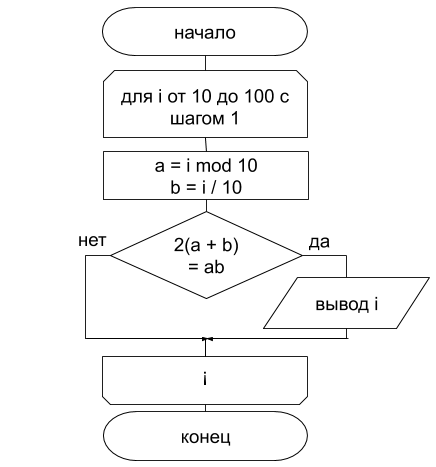
\includegraphics[scale=0.6]{lab2-4.png}\\
Схема программы
\end{center}
\lstinputlisting[language=c, frame=single, caption=Программа четвертого задания, label=lab2_2, style=CStyle]{../fourthTask.c}
\begin{center}
Текст программы
\end{center}
\begin{center}
\begin{tabular}{|p{7cm}|p{7cm}|}
\hline
\multicolumn{1}{|c|}{Исходные данные}& \multicolumn{1}{|c|}{Вывод программы}\\
\hline
Ввода не требуется & 36 44 63\\
\hline
\end{tabular}\\
\vspace{0.3cm}
Результаты тестирования
\end{center}

\subsection{Задание 5}
Несколько деталей должны последовательно пройти обработку на каждом из трех станков. Продолжительности обработки каждой детали на каждом станке вводятся группами по три числа до исчерпания ввода (признак окончания ввода – задание некорректной тройки чисел). Сколько времени займет обработка всех деталей, если на каждом станке они могут обрабатываться только поштучно?\\
\textit{Исходные данные:} Вводимые значения могут быть любыми, поэтому нужно объявить их типа double.\\
\textit{Результирующие данные:} Общая сумма так же типа double.\\
\begin{center}
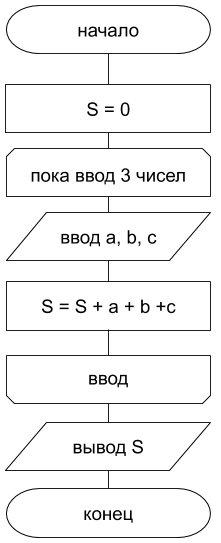
\includegraphics[scale=0.6]{lab2-5.png}\\
Схема программы
\end{center}
\lstinputlisting[language=c, frame=single, caption=Программа пятого задания, label=lab2_2, style=CStyle]{../fivthTask.c}
\begin{center}
Текст программы
\end{center}
\begin{center}
\begin{tabular}{|l|l|}
\hline
\multicolumn{1}{|c|}{Исходные данные}& \multicolumn{1}{|c|}{Вывод программы}\\
\hline
a,b,c = 1,2,3 | 3,4,5 | b & 18.000000\\
a,b,c = 7,3,6 | 4,a & 16.000000\\
a,b,c = 3,3,3 | 30,2,5 | b,4,4 & 46.000000\\
\hline
\end{tabular}\\
\vspace{0.3cm}
Результаты тестирования
\end{center}

\subsection{Задание 6}
Получить число, образованное записью цифр исходного числа N в обратном порядке.\\
\textit{Исходные данные:} Введеное число может быть больших размеров, но обязательно будет целым, поэтому используем тип long int для объявления n.\\
\textit{Результирующие данные:} Отдельной переменной не требуется.\\
\textit{Дополнительные переменные:} Для хранения развернутого числа объявим переменную b типа так же long int.\\
\begin{center}
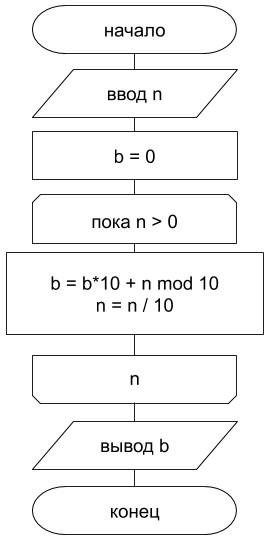
\includegraphics[scale=0.6]{lab2-6.png}\\
Схема программы
\end{center}
\lstinputlisting[language=c, frame=single, caption=Программа шестого задания, label=lab2_2, style=CStyle]{../sixthTask.c}
\begin{center}
Текст программы
\end{center}
\begin{center}
\begin{tabular}{|l|l|}
\hline
\multicolumn{1}{|c|}{Исходные данные}& \multicolumn{1}{|c|}{Вывод программы}\\
\hline
n = 912364 & b = 463219\\
n = 913269412 & b = 214962319\\
n = 8172374162734 & b = 4372614732718\\
\hline
\end{tabular}\\
\vspace{0.3cm}
Результаты тестирования
\end{center}

\subsection{Задание 7}
Вычислить значение суммы бесконечного ряда\\
$f(x) = 1 - \displaystyle\frac{x^2}{2!} + \frac{x^4}{4!} - ... + \frac{(-1)^nx^{2n}}{(2n)!} + ...$\\
с заданной точностью e = $10^{-5}$ и значение функции (для проверки) y = cosx. 
\textit{Исходные данные:} Введеное число может быть больших размеров поэтому используем тип double для x.\\
\textit{Результирующие данные:} Сумма элементов будет хранится в S типа double.\\
\textit{Дополнительные переменные:} Для ускорения работы программы введем переменные типа double x2, для хранения квадрата x, n2, для хранения квадрата n, a, для хранения n-ого элемента последовательности. В качестве счетчика элементов последовательности используем n типа int.\\
\begin{center}
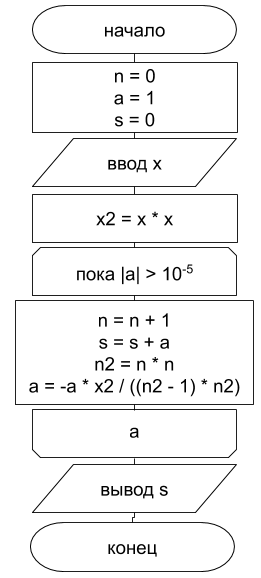
\includegraphics[scale=0.6]{lab2-7.png}\\
Схема программы
\end{center}
\lstinputlisting[language=c, frame=single, caption=Программа седьмого задания, label=lab2_2, style=CStyle]{../seventhTask.c}
\begin{center}
Текст программы
\end{center}
\begin{center}
\begin{tabular}{|l|l|l|}
\hline
\multicolumn{1}{|c|}{Исходные данные}&\multicolumn{1}{|c|}{cos(x)}& \multicolumn{1}{|c|}{Вывод программы}\\
\hline
x = 12 & 0.843855 & s = 0.843854\\
x = 4 & -0.653644 & s = -0.653644\\
x = -9 & -0.911130 & s = -0.911129\\
\hline
\end{tabular}\\
\vspace{0.3cm}
Результаты тестирования
\end{center}

\subsection{Задание 8}
Вычислить значение суммы членов бесконечного ряда\\
$S = ln x + \displaystyle2[\frac {a} {2x+a} + \frac {a^3} {3(2x+a)^3} + \frac {a^5} {5(2x+a)^5}
+ ... + \frac {a^{2n-1}} {(2n-1)(2x+a)^{2n-1}} + ...]$\\
c точностью до члена ряда, меньшего  e = $10^{-4}$ для $a^2<(2x+a)^2$, и значение функции (для проверки) f = ln(x+a).\\
\textit{Исходные данные:} Введеные числа могут быть больших размеров поэтому используем тип double для x и a.\\
\textit{Результирующие данные:} Сумма элементов будет хранится в S типа double.\\
\textit{Дополнительные переменные:} Для ускорения работы программы введем переменные типа double x2, для хранения квадрата x, b, для хранения n-ого элемента последовательности, k, для хранения коэфициента частного между элементами последовательности. В качестве счетчика элементов последовательности используем n типа int.\\
\begin{center}
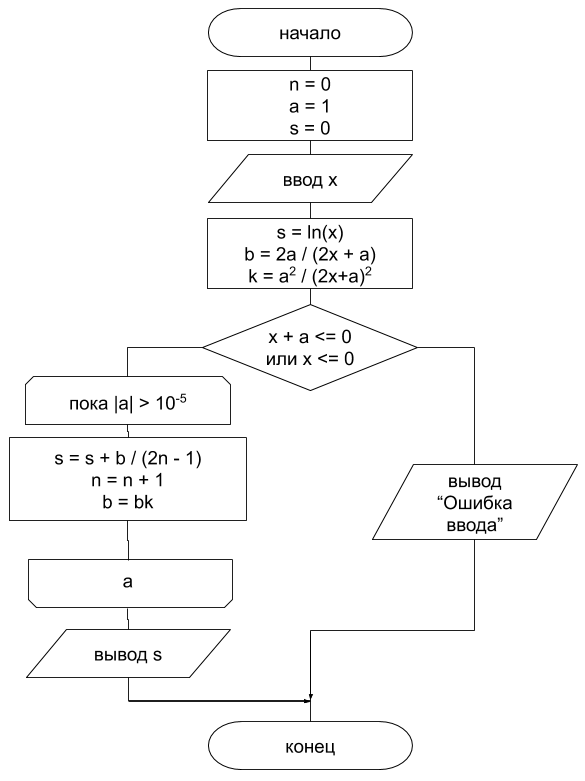
\includegraphics[scale=0.6]{lab2-8.png}\\
Схема программы
\end{center}
\lstinputlisting[language=c, frame=single, caption=Программа восьмого задания, label=lab2_2, style=CStyle]{../eightTask.c}
\begin{center}
Текст программы
\end{center}
\begin{center}
\begin{tabular}{|l|l|l|}
\hline
\multicolumn{1}{|c|}{Исходные данные}&\multicolumn{1}{|c|}{ln(x + a)}& \multicolumn{1}{|c|}{Вывод программы}\\
\hline
x = 4, a = 6 & 2.30259 & s = 2.30258\\
x = -3, a = 4 & Недопустимое значение & Недопустимое значение\\
x = 9, a = -2 & 1.94591 & s = 1.94591\\
\hline
\end{tabular}\\
\vspace{0.3cm}
Результаты тестирования
\end{center}

\subsection{Задание 9}
Вычислить:\\
\begin{center}
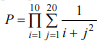
\includegraphics[scale=1]{formula.png}
\end{center}
\textit{Исходные данные:} Считывать пользовательский ввод не требуется.\\
\textit{Результирующие данные:} Произведение сумм элементов будет хранится в P типа double.\\
\textit{Дополнительные переменные:} Счетчиками циклов взяты i и j типа char, вспомогательная перменная для хранения суммы элементов вложенного цикла - a, типа double.\\
\begin{center}
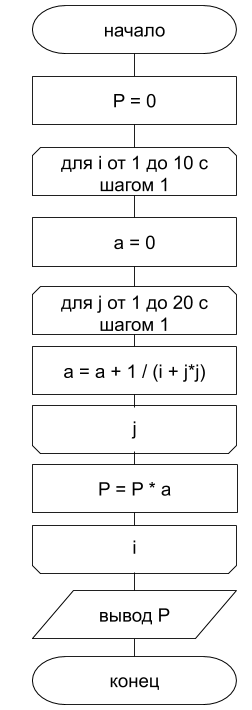
\includegraphics[scale=0.6]{lab2-9.png}\\
Схема программы
\end{center}
\lstinputlisting[language=c, frame=single, caption=Программа девятого задания, label=lab2_2, style=CStyle]{../ninthTask.c}
\begin{center}
Текст программы
\end{center}
\begin{center}
\begin{tabular}{|p{7cm}|p{7cm}|}
\hline
\multicolumn{1}{|c|}{Исходные данные}& \multicolumn{1}{|c|}{Вывод программы}\\
\hline
Ввод не требуется & P = 0.003508\\
\hline
\end{tabular}\\
\vspace{0.3cm}
Результаты тестирования
\end{center}


\end{document}
